\chapter{المتجهات}

\section{مقدمة}
المتجهات او ما يطلق عليها الكمية المتجهة هي طريقة يتم من خلالها قياس الكميات والتعرف على مقادير الاشياء. وقد تكون معرفة الكمية المتجهة من الامور الطبيعية في حياتنا والتي لها فوائد متعددة في جميع المجالات الحياتية

\section[تعريف المتجهات]{تعريف المتجهات \cite{key1}}
هي كميات رياضية لها مقدار واتجاه. تستخدم المتجهات في العديد من المجالات مثل: الملاحة والطيران والطقس. تتميز المتجهات بخصائص مثل: الجمع والطرح والضرب.

\section{العمليات على المتجهات (العمليات الجبرية)}
\subsection*{1. جمع المتجهات}
عند جمع متجهين معاً يصبح عندها متجه جديد يختلف عنهما بالمقدار والاتجاه. ويمكن التعبير عن ذلك بالعلاقة
\begin{align*}
	\vec{U} + \vec{V} &= (U_1, U_2, \dots, U_n) + (V_1, V_2, \dots, V_n)\\
	&= (U_1+V_1, U_2+V_2, \dots, U_n+V_n)
\end{align*}
الشكل \ref{fig:vecsum} يبين التمثيل الهندسي لعملية جمع المتجهات.
	\begin{figure}[ht]
	\centering
	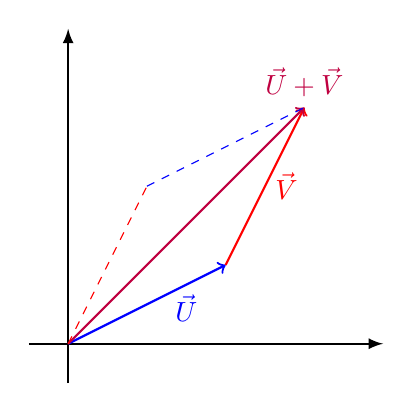
\begin{tikzpicture}
		\draw[thick, -latex] (-0.5, 0) -- (4, 0);
		\draw[thick, -latex] (0, -0.5) -- (0, 4);
		
		\draw[thick, blue, ->] (0,0) -- (2,1) node[pos=.75, below]{$\vec{U}$};
		\draw[thick, red, ->] (2,1) -- ++(1,2) node[midway, right]{$\vec{V}$};
		
		\draw[->, thick, purple] (0, 0) -- (3,3) node[above] {$\vec{U}+\vec{V}$};
		
		\draw[dashed, red] (0, 0) -- (1,2);
		\draw[dashed, blue] (1,2) -- (3,3);
	\end{tikzpicture}
	\caption{التمثيل الهندسي لجمع النتجهات}
			\label{fig:vecsum}
\end{figure}
\newpage
\begin{example}
لجمع المتجهين
	
	$\vec{W} = (3,-2)$ و $\vec{V} = (5,4)$
	نتبع الخطوات التالية
	\begin{align*}
		\vec{W} + \vec{V} &= (5,4) + (3,-2)\\
		&= (5+3, 4-2)\\
		&= (8,2)
	\end{align*}
\end{example}


\subsection*{2. طرح المتجهات}
يعطى بالعلاقة التالية
\[
\vec{U} - \vec{V} = \vec{U} + (-\vec{V})
\]
الشكل \ref{fig:vecdiff} يبين التمثيل الهندسي لطرح المتجهات.
	\begin{figure}[ht]
	\centering
	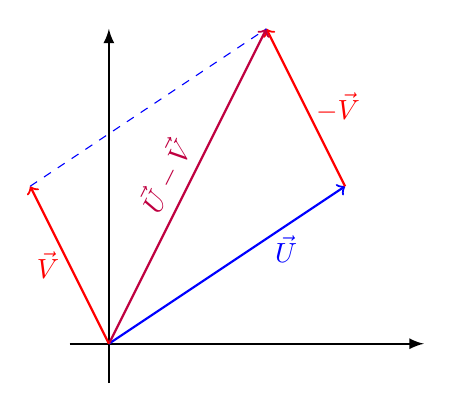
\begin{tikzpicture}
		\draw[thick, -latex] (-0.5, 0) -- (4, 0);
		\draw[thick, -latex] (0, -0.5) -- (0, 4);
		
		\draw[thick, blue, ->] (0,0) -- (3,2) node[pos=.75, below]{$\vec{U}$};
		\draw[thick, red, ->] (0,0) -- (-1,2) node[midway, left]{$\vec{V}$};
		
		\draw[thick, red, ->] (3, 2) -- ++(-1, 2) node[pos=.5, right]{$-\vec{V}$}; 
		
		\draw[thick, purple, ->] (0,0) -- (2, 4) node[midway, sloped, above]{$\vec{U} - \vec{V}$};
		
        \draw[dashed, red] (0, 0) -- (-1, 2);
        \draw[dashed, blue](-1, 2) -- ++(3,2);
		
	\end{tikzpicture}
	\caption{التمثيل الهندسي لطرح النتجهات}
	\label{fig:vecdiff}
\end{figure}

\begin{example}
	ليكن
	$\vec{V}=(5, 7), \vec{W} = (4,2)$
	فإن 
	\begin{align*}
		\vec{V}-\vec{W} &= (5,7) + (-4, -2)\\
		&= (5-4, 7-2)\\
		&= (1,5)
	\end{align*}
\end{example}
\noindent
اي بمعنى اخذ النظير الجمعي للمتجه الثاني وتصبح العملية كأنها عملية جمع.

\subsection*{3. ضرب عدد في متجه}
عند ضرب عدد في متجه يتغير الطول فقط. وعند ضرب المتجه في عدد سالب يتغير الاتجاه، للتعبير عنه يعطى بالعلاقة التالية
\begin{align*}
	k \vec{U} &= k(U_1, U_2, \dots, U_n)\\
	&= (kU_1, kU_2, \dots, kU_n)
\end{align*}

\begin{example}
	جد ناتج $12\vec{V}$ حيث $\vec{V}=(1,-9,0,2)$
\end{example}
\noindent
\textbf{الحل}\\
\noindent
$k=12, \vec{V}=(1,-9,0,2)$
\begin{align*}
	k\vec{V} &= 12(1,-9,0,2)\\
	&= (12\times1, 12\times-9, 12\times0, 12\times2)\\
	&= (12, -108, 0, 24)
\end{align*}

\section[خواص المتجهات]{خواص المتجهات \cite{key2}}
لتكن $\vec{U}, \vec{V}, \vec{W}$ متجهات في $\R^n$ و $c,k$ ثوابت
\begin{english}
	\begin{enumerate}
		\item $\vec{U} + \vec{V} = \vec{V} + \vec{U}$
		\item $(\vec{U} + \vec{V} )+ \vec{W} = \vec{U} + (\vec{V} + \vec{W})$
		\item $\vec{U}+\vec{0} = \vec{0} + \vec{U} = \vec{U}$
		\item $\vec{U} + (\vec{-U}) = \vec{0}$
		\item $(ck)\vec{U} = c(k\vec{U})$
		\item $k(\vec{U}+\vec{V}) = k\vec{U} + k\vec{V}$
		\item $(c+k)\vec{U} = c\vec{U} + k\vec{U}$
		\item $1\cdot \vec{U} = \vec{U}$
	\end{enumerate}
\end{english}

\section[متجه الوحدة]{متجه الوحدة \cite{key1}}
هو متجه ذو مقدار وحدة واحدة، يستخدم عادةً للاشارة الى الاتجاه. يعطى بالعلاقة التالية
\[
\vec{U} = \frac{1}{|| \vec{V}||}\cdot \vec{V}
\]

\begin{example}
	ليكن $\vec{W}=(4,-2,1)$ متجه. جد متجه الوحدة
\end{example}
\noindent
\textbf{الحل}
\[
\vec{U} = \frac{1}{|| \vec{W}||}\cdot \vec{W}
\]
\begin{align*}
	||W|| &= \sqrt{4^2 + (-2)^2 + 1^2}\\
	& = \sqrt{16 + 4 +1}\\
	&= \sqrt{21}
\end{align*}
\begin{align*}
	\vec{U} = \frac{1}{\sqrt{21}}\cdot(4,-2,1) = \left(\frac{4}{\sqrt{21}}, \frac{-2}{\sqrt{21}}, \frac{1}{\sqrt{21}}\right)
\end{align*}

\section[الضرب العددي النقطي]{الضرب العددي النقطي \cite{key3}}
ليكن $\vec{U}, \vec{V}$ متجهين في $\R^n$ فإن الضرب النقطي لهما يعطى بالعلاقة 
\[
\vec{U} \cdot \vec{V} = u_1v_1 + u_2v_2 + \cdots + u_nv_n
\]
\noindent
لضرب متجهين جبرياً نقطياً. نقوم بضرب العدد الاول من المتجه الاول في العدد الاول من المتجه الثاني، العدد الثاني من المتجه الاول في العدد الثاني من المتجه الثاني وهكذا\dots
\begin{example}
	ليكن 
	$\vec{U} = (-8, 0, -12), \vec{V}=(5,7,1)$
	اوجد $\vec{U}\cdot\vec{V}$.
\end{example}
\noindent
\textbf{الحل}
\begin{align*}
	\vec{U}\cdot\vec{V} &= u_1v_1 + u_2v_2 + u_3v_3\\
	&= (-8)(5) + (0)(7) + (-12)(1)\\
	&= -40 + 0 -12\\
	&= -52
\end{align*}

\subsection*{خواص الضرب النقطي}

\begin{english}
	\begin{enumerate}
		\item $\vec{U}\cdot\vec{V}=\vec{V}\cdot\vec{U}$
		\item $\vec{U}\cdot(\vec{V}+\vec{W}) = \vec{U}\cdot\vec{V} + \vec{U}\cdot\vec{W}$
		\item $k(\vec{U}\cdot\vec{V}) = (k\vec{U})\cdot\vec{V}$
		\item $\vec{V}\cdot\vec{V} = ||\vec{V}||^2$
		\item $\vec{V}\cdot \vec{0} = \vec{0}$
	\end{enumerate}
\end{english}

\section[الزاوية بين المتجهين]{الزاوية بين المتجهين \cite{key2}} 
تعطى بالعلاقة التالية
\[
\cos\alpha = \frac{\vec{U}\cdot\vec{V}}{||\vec{U}|| \cdot ||\vec{V}||}
\]
من العلاقة السابقة نستطيع ان نحصل على
\[
\vec{U}\cdot\vec{V} = ||\vec{U}|| \cdot||\vec{V}||\cdot \cos \alpha
\]

\begin{example}
	ليكن 
	$\vec{U}=(1,0,0), \vec{V}=(0,0,1)$
	جد الزاوية بين هذين المتجهين 
\end{example}
\noindent
\textbf{الحل}
\begin{align*}
	\vec{U}\cdot\vec{V} &= u_1v_1 + u_2 v_2 + u_3 v_3\\
	&= (1)(0) + (0)(0) + (0)(1)\\
	&= 0+0+0=0
\end{align*}
\[
||\vec{U}|| = \sqrt{1^2 + 0^2 + 0^2} = \sqrt{1} =1
\]
\[
||\vec{V}|| = \sqrt{0^2 + 0^2 + 1^2} = \sqrt{1} =1
\]
\[
\cos\alpha = \frac{\vec{U}\cdot\vec{V}}{||\vec{U}|| \cdot ||\vec{V}||} =  \frac{0}{1} = 0
\]
\[
\Rightarrow \alpha =\frac{\pi}{2}
\]

\section[الضرب الاتجاهي]{الضرب الاتجاهي \cite{key4}}
ليكن $\vec{U}, \vec{V}$ متجهين في $\R^3$ فإن الضرب الاتجاهي لهما يكون كالاتي
\begin{align*}
	\vec{U}\times\vec{V} & = 
	\begin{vmatrix}
		i & j & k\\
		U_1 & U_2 & U_3\\
		V_1 & V_2 & V_3
	\end{vmatrix}\\
	&= i(U_2V_3 - U_3V_2 ) -j(U_1V_3 - U_3V_1) + k(U_1V_2 - U_2V_1)
\end{align*}
\begin{example}
	ليكن
	$\vec{U} = (2,3,-2), \vec{V} = (1,-1,0)$ 
	اوجد $\vec{U}\times\vec{V}$
\end{example}
\noindent
\textbf{الحل}
\begin{align*}
	\vec{U}\times\vec{V} & = 
	\begin{vmatrix}
		i & j & k\\
		2 & 3 & -2\\
		1 & -1 & 0
	\end{vmatrix}\\
	&= i[(3)(0) - (-2)(-1)] -j[(2)(0) - (-2)(1)] + k[(2)(-1) -(3)(1)]\\
	&= i(0-2) - j(0+2) + k(-2-3)\\
	&= -2i -2j -5k
\end{align*}

\subsection*{خصائص الضرب الاتجاهي}
\begin{english}
	\begin{enumerate}
		\item $\vec{U}\times\vec{V} = -(\vec{V}\times\vec{U})$
		\item $\vec{U}\times(\vec{V} + \vec{W}) = (\vec{U}\times\vec{V}) + (\vec{U}\times\vec{V})$
		\item $(\vec{U}+\vec{V})\times\vec{W} = (\vec{U}\times\vec{W}) + (\vec{U}\times\vec{W})$
		\item $c(\vec{U}\times\vec{V}) = (c\vec{U})\times\vec{V} = \vec{U}\times(c
		\vec{V})$
		\item $\vec{U}\times\vec{0} = \vec{0}\times\vec{U} = \vec{0}$
		\item $\vec{U}\times\vec{U} = \vec{0}$
	\end{enumerate}
\end{english}
\noindent
\subsection*{متطابقة لاكرانج}
\[
||\vec{U}\times\vec{V}||^2 = ||\vec{U}||^2 \cdot ||\vec{V}|| - (\vec{U}\cdot\vec{V})^2
\]

\begin{example}
	ليكن
	$\vec{U}=(-2, 1,0) , \vec{V}=(4,2,-5)$
	طبق متطابقة لاكرانج عليهما
\end{example}
\noindent
\textbf{الحل}
\begin{align*}
		\vec{U}\times\vec{V} & = 
	\begin{vmatrix}
		i & j & k\\
		-2 & 1 & 0\\
		4 & 2 & -5
	\end{vmatrix}\\
	&= i(-5-0) - j(10-0) + k(-4-4)\\
	&= -5i -10j -8k
\end{align*}

\begin{align*}
	||\vec{U}\times\vec{V}||^2 &= (-5)^2 + (-10)^2 + (-8)^2\\
	&= 25 + 100 + 64 \\
	&= 189
\end{align*}
\begin{align*}
	||\vec{U}||^2 &= (-2)^2 + 1^2 + 0^2\\
	&= 4+1+0\\
	&= 5
\end{align*}
\begin{align*}
	||\vec{V}|| &= 4^2 + 2^2 + (-5)^2\\
	&= 16 + 4 + 25\\
	&= 45
\end{align*}
\begin{align*}
	(\vec{U}\cdot\vec{V})^2 &= [(-2,1,0)\cdot(4,2,-5)]^2\\
	&= (-8+2+0)^2\\
	&= (-6)^2\\
	&= 36
\end{align*}
نطبق العلاقة 
\begin{gather*}
	189 = 5\times 45 - 36\\
	189 = 225 - 36\\
	 189 = 189
\end{gather*}
اذن نلاحظ ان الطرف الايمن يجب ان يساوي الطرف الايسر لكي يحقق المتطابقة.


